% IRSpectra-Bench --- ICLR conference manuscript (Overleaf / tectonic / XeLaTeX)
% Style: official ICLR 2026 conference macros (vendored as iclr2026_conference.sty).
% Working notes: docs/ICLR_PAPER.md
%
% Overleaf: set main document to docs/iclr/iclr_paper.tex (this copy) or
% IRSpectra-Bench repo root (postcard). Headline n=295 generation; fverify n=194.
% Compile with pdfLaTeX or XeLaTeX + BibTeX (references.bib + iclr2026_conference.bst).
% \iclrfinalcopy is the only official sty flag that prints \author and drops
% the left-margin submission ruler (see tex/iclr2026_conference.sty).
\documentclass{article}
\usepackage{iclr2026_conference,times}

\usepackage{hyperref}
\usepackage{url}
\usepackage{booktabs}
\usepackage{graphicx}
\usepackage{amsmath,amssymb}
\usepackage{enumitem}
\setlist{nosep,leftmargin=1.35em}

\graphicspath{{figures/}{../figures/}{./}}

\title{Generation Recall, Not Verification, Binds LLM Structure Elucidation from Literature Spectra}

\author{
Ilkham Yabbarov\textsuperscript{1,$\dagger$},
Rudra Sondhi\textsuperscript{1},
Rodrigo A.\ Vargas-Hern\'andez\textsuperscript{1,2,3,$\dagger$}\\
\textsuperscript{1}Department of Chemistry and Chemical Biology, McMaster University,
Hamilton, Ontario L8S 4L8, Canada.\\
\textsuperscript{2}Brockhouse Institute for Materials Research, McMaster University,
Hamilton, Ontario L8S 4L8, Canada.\\
\textsuperscript{3}School of Computational Science and Engineering, McMaster University,
Hamilton, Ontario L8S 4L8, Canada.\\
$\dagger$\,\textit{E-mail:} yabbaroi@mcmaster.ca, vargashr@mcmaster.ca
}

\newcommand{\fix}{\marginpar{FIX}}
\newcommand{\new}{\marginpar{NEW}}

% Official ICLR 2026 switch: show \author and disable the submission linenumber
% ruler. The same flag also sets the running header to "Published as...".
% Double-blind (submit): keep \iclrfinalcopy commented; \maketitle then prints
% "Anonymous authors / Paper under double-blind review". Camera-ready: uncomment
% \iclrfinalcopy and delete the \lhead override below.
% \iclrfinalcopy  % OFF for double-blind submission; re-enable for camera-ready
\begin{document}

\maketitle
\lhead{Under review as a conference paper at ICLR 2026}

\begin{abstract}
Frontier large language models are often presented as near-solved structure elucidators on
curated spectra. We ask a harder, more operational question: given the molecular formula and
\textbf{literature-reported} IR / $^1$H / $^{13}$C \textbf{peak lists} --- not digitised traces ---
can an off-the-shelf LLM recover the correct constitution, and \textbf{which stage fails} when
it does not?

We introduce \textbf{IRSpectra-Bench}, a blind, mechanically scored peak-list benchmark of 295
compounds (194 locked $+$ 101 spectrally-clean expansion; five $^{13}$C-overread records
excluded before scoring) drawn from redistributable experimental band lists (\textbf{IRexp}; companion Data
Descriptor)~\citep{yabbarov2026irexp}, with a fixed RDKit InChIKey-connectivity scoring contract
and decomposable \textbf{generation recall} / \textbf{verification precision} metrics.
On IRSpectra-Bench, a frontier LLM recovers the correct constitution for \textbf{39\%} top-1
(116/295; 95\% CI 34--45), or \textbf{27\%} once reweighted to corpus composition; generation
recall is \textbf{44\%} (130/295).
The bottleneck is \textbf{candidate proposal, not verification}: on the $n{=}194$ slice with
forward-verification, the true structure enters the pool for only \textbf{34\%} of compounds,
and where it does, training-free forward-verification selects it \textbf{89\%} of the time (58/65).
Expansion forward-verify is pending.
The same recall $\ll$ precision asymmetry replicates across \textbf{four vendor families}.
A formula-only control ($n{=}60$) drops top-1 from 23\% $\to$ 5\%; accuracy is flat in source-paper year
on the locked slice.
Generate-wide sampling on that arm lifts recall 32\% $\to$ 42\% and top-1 23\% $\to$ 30\%, while
verification alone moves $n{=}194$ top-1 only 28\% $\to$ 30\%.
Recovered from published top-$k$ figures, recall carries \textbf{68--83\%} of the accuracy
collapse when systems move from curated or simulated data to real heterogeneous spectra.
Frozen predictions, scorers and code are released for mechanical re-evaluation.
\end{abstract}

\section{Introduction}
\label{sec:introduction}

Structure elucidation from spectra sits at the centre of synthetic and analytical chemistry,
and machine learning increasingly treats it as a sequence or agent task.
Encoder--decoder models train on paired corpora~\citep{chacko2024spectro,ottomano2025nmiracle,alberts2024ir};
LLM agents and puzzle benches report high recovery on curated or education
spectra~\citep{kamber2026chemist,guo2024molpuzzle,zhuang2025treesearch,espejo2026agentic}.
Cross-paper numbers swing wildly with harness (e.g.\ GPT-4o from 1.4\% to 57.8\% on MolPuzzle
under different prompting~\citep{guo2024molpuzzle,zhuang2025treesearch}).
What remains under-measured is the chemist's operational task: \textbf{taking peak lists as
printed in open-access papers and recovering constitution}, with a fixed molecular-representation
scoring contract and an honest account of \textbf{which stage of elucidation binds}.

We argue that end-to-end top-1 alone is the wrong reporting primitive.
Any system that returns a ranked candidate list factorises as
\begin{equation}
\text{top-1} \;=\; \underbrace{P(\text{true} \in \text{pool})}_{\text{generation recall}}
\times
\underbrace{P(\text{rank}=1 \mid \text{true} \in \text{pool})}_{\text{verification precision}}.
\end{equation}
These rates have different denominators and must not be differenced.
Prior work already notes that re-ranking cannot recover a missing
candidate~\citep{priessner2026reasoning}; we supply the missing \textbf{measurement
infrastructure at scale}.

\paragraph{Contributions.}
\begin{enumerate}
  \item \textbf{IRSpectra-Bench} --- a blind, complexity-stratified peak-list benchmark ($n{=}295$)
        with a pre-registered InChIKey-connectivity scorer and community reporting contract
        (top-1, generation recall, verification precision $|$ recall).
  \item \textbf{A recall-bound diagnosis} on a frontier LLM: 44\% proposed on the pooled generation
        cohort; on the $n{=}194$ forward-verified slice, 34\% proposed and 89\% selected once
        proposed; that slice's top-1 moves only 28\% $\to$ 30\% under training-free
        forward-verification. Expansion forward-verify is pending.
  \item \textbf{Contamination and cross-vendor controls} --- formula-only and recency bounds;
        four-vendor replication of recall $\ll$ precision.
  \item \textbf{A literature decomposition} that recovers the same split from published top-$k$
        figures, showing recall carries most of the collapse on real heterogeneous data.
\end{enumerate}

\paragraph{Dataset pointer (not this paper's primary object).}
Experimental band lists come from \textbf{IRexp} (121,233 records; 43,060 structure-linked;
33,201 full IR+$^1$H+$^{13}$C+structure quadruples); an anonymised review copy is linked in Appendix~\ref{app:dataset}.
Construction, licensing, and technical validation of the corpus are the subject of a companion
\textit{Scientific Data} manuscript (in preparation)~\citep{yabbarov2026irexp}.
This ICLR paper \textbf{cites} that resource and does not re-present a Data Descriptor.

\begin{figure}[t]
  \centering
  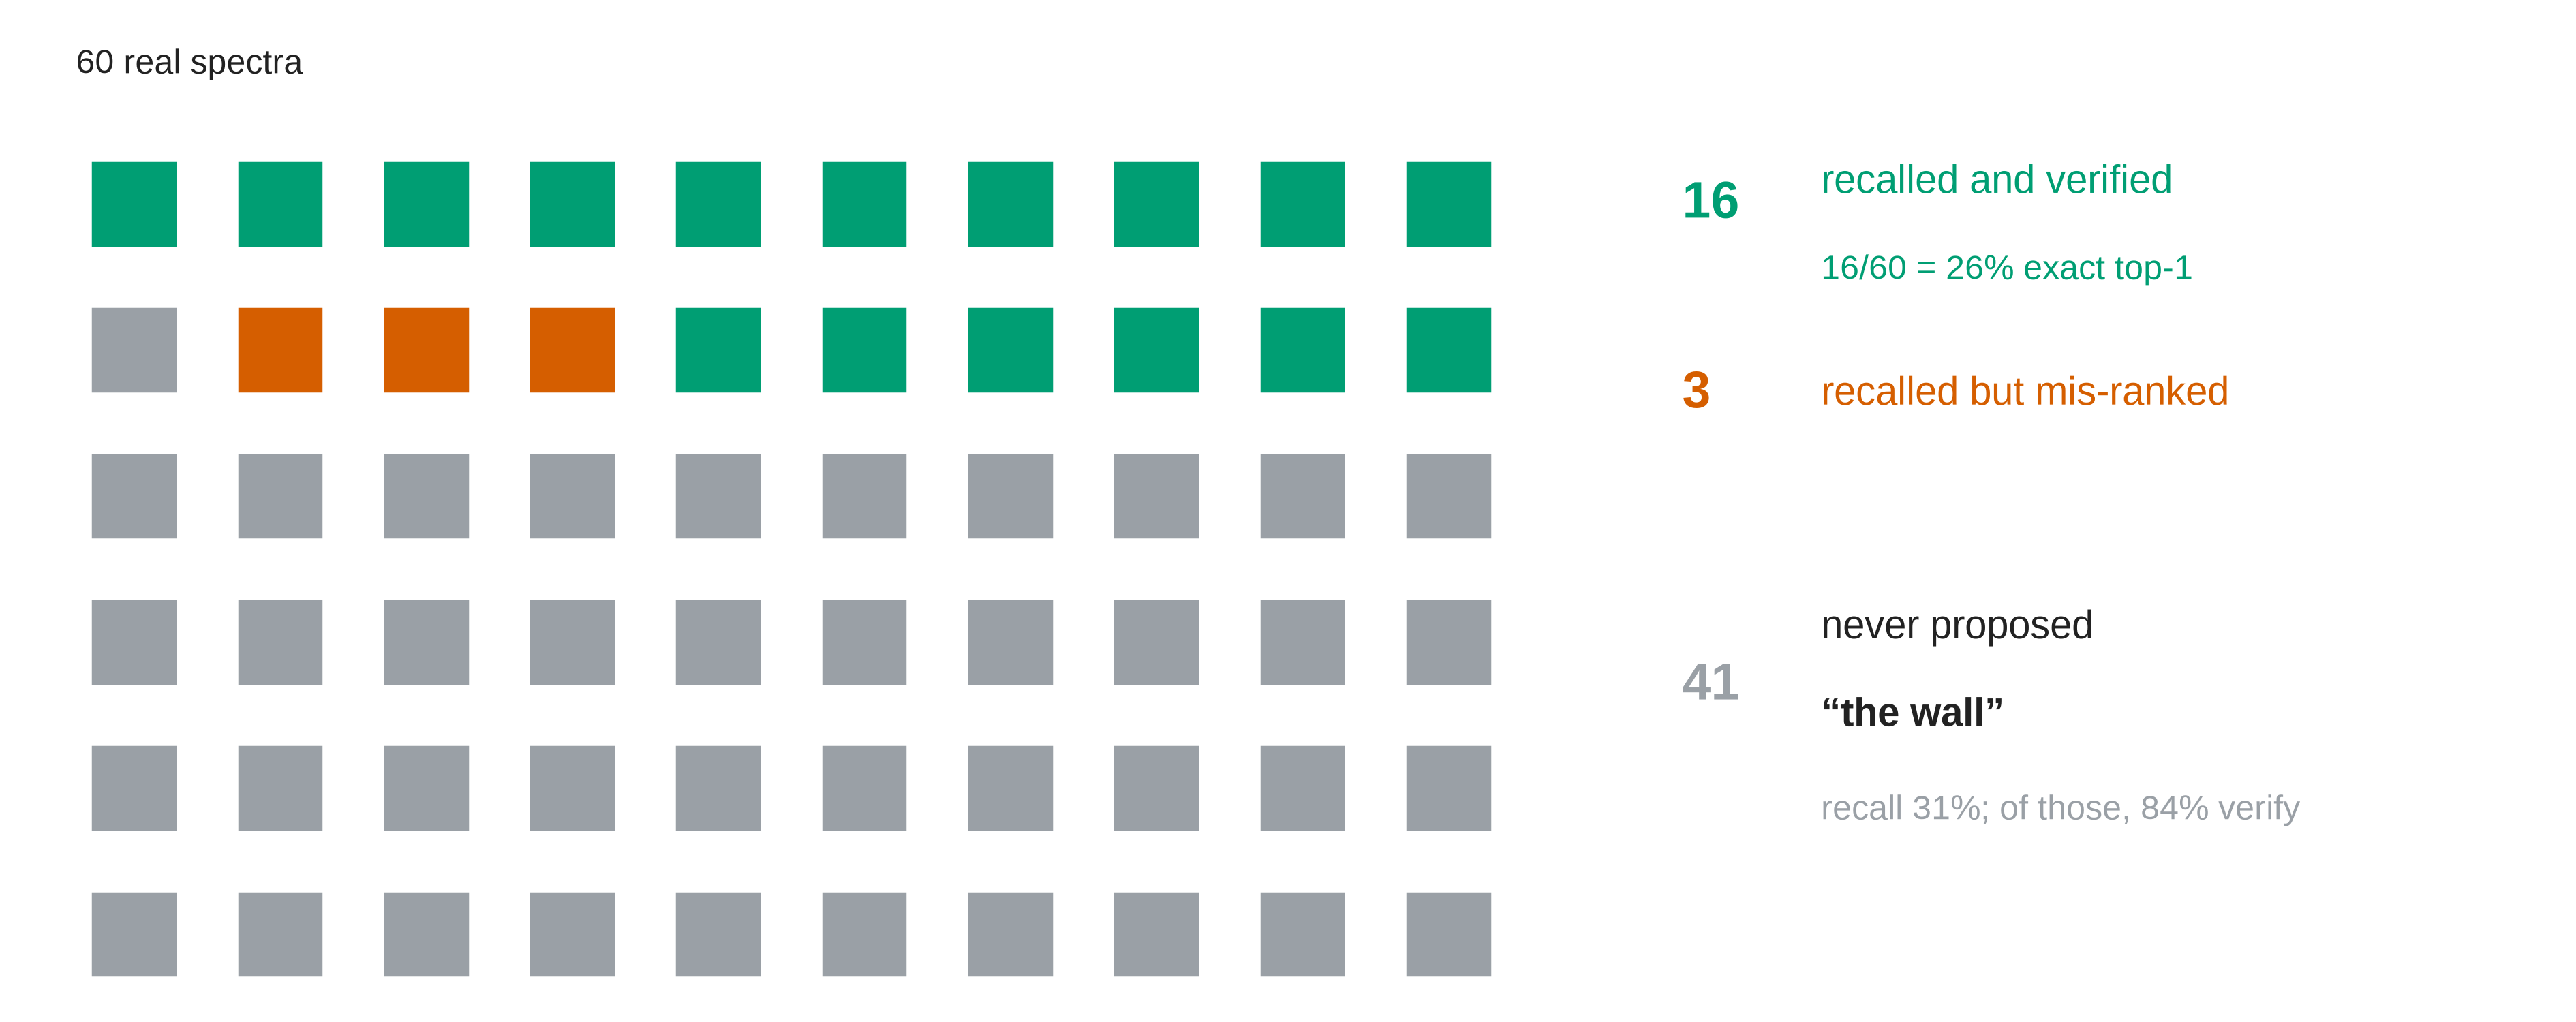
\includegraphics[width=\linewidth]{fig_wall.png}
  \caption{Forward-verified diagnosis on the locked IRSpectra-Bench slice ($n{=}194$;
  58 verified / 7 mis-ranked / 129 never proposed). Generation recall on the pooled
  headline ($n{=}295$) is 130/295 (44\%); expansion forward-verify is pending, so this
  plate is not a pooled wall. Where the true structure is never proposed, no ranker can
  recover it; where it is proposed, verification usually selects it.}
  \label{fig:fig-wall}
\end{figure}

\section{Related work}
\label{sec:related-work}

\paragraph{Trained spectra $\to$ structure models.}
Sequence and graph decoders on paired
corpora~\citep{chacko2024spectro,hu2024multitask,yang2026nmrtrans,ottomano2025nmiracle,alberts2024ir,alberts2025benchmarks}
are accurate in-distribution but typically scored end-to-end.
We do not claim to beat them on IRSpectra-Bench; Spectro, NMIRacle, Alberts IR transformers
and CASE are \textbf{not yet scored} on our bench (Section~\ref{sec:limitations}) --- a gap we
state honestly and leave to the released scorer.

\paragraph{LLM agents and puzzle benches.}
ChemCrow~\citep{mbran2024chemcrow}, Coscientist~\citep{boiko2023coscientist},
SpectralLM~\citep{su2025spectrallm}, SpecMol~\citep{shen2025specmol}, tree-search
elucidation~\citep{zhuang2025treesearch}, IR-Agent~\citep{noh2025iragent} and Priessner
\textit{et al.}~\citep{priessner2026reasoning} improve \emph{how} a model reads spectra or
re-ranks a fixed pool.
We fix one protocol and ask \textbf{which stage binds} once the spectra have been read.

\paragraph{Contamination-aware and heterogeneous-data benches.}
Most prior suites use simulated or single-instrument spectra.
IRSpectra-Bench uses literature-reported peak lists across thousands of laboratories and
reports formula-only and recency controls (Section~\ref{sec:contamination}).
Espejo Morales \textit{et al.}~\citep{espejo2026agentic} compare education vs industrial
\emph{instrument files} (80.9\% $\to$ 20.6\%); they ask which architecture, while we ask which stage
binds on \textbf{published reports}.

\paragraph{Forward verification and CASE.}
Matching predicted to observed shifts --- DP4~\citep{smith2010dp4},
CASE~\citep{elyashberg2012case}, NMR-Solver~\citep{jin2025nmrsolver},
NMRAgent~\citep{fang2026nmragent} --- is easier than inverse generation.
CASE enumerators have exhaustive recall by construction; the LLM literature almost never
reports whether the true structure was proposed at all.
We decompose error rather than chase a single top-1.

\paragraph{Positioning.}
Concurrent 2026 suites (MolQuest~\citep{han2026molquest}, SpecX~\citep{xiang2026specx},
NMRGym~\citep{fang2026nmrgym}) bound related tasks.
IRSpectra-Bench is an openly redistributable suite on literature peak lists with a \textbf{stage
decomposition} measured on Claude and replicated across three other model families.

\section{IRSpectra-Bench}
\label{sec:benchmark}

\subsection{Task and inputs}

Each of 295 problems supplies the \textbf{molecular formula} (as from HRMS), the \textbf{IR
band list} (cm$^{-1}$), and \textbf{$^1$H / $^{13}$C shift lists} --- exactly the textual form
reported in open-access papers.
No name, SMILES or scaffold hint.
Inputs are author-transcribed \textbf{band and shift lists}, not absorbance traces or FIDs:
a different object from digitised-spectrum benchmarks~\citep{espejo2026agentic}, and one that
matches how language models consume literature.

The cohort is the pre-registered pool of a locked 194 (spectrally validated main round 134 $+$
60 controls) and a 106-compound expansion draw; five expansion records fail the same
$^{13}$C-overread audit used on the main round and are excluded from the headline
($n{=}295{=}194{+}101$), not scored away after seeing the result.
Problems are drawn from the structure-complete split of IRexp (\texttt{irexp\_resolved}; see
companion Data Descriptor)~\citep{yabbarov2026irexp}.
On the locked 194, author peak assignments name a ring system in 10/194; those are solved
1/10 vs 54/184 for the rest, so named-ring annotation does not drive that slice.

\subsection{Difficulty, balance, and scoring contract}

\textbf{Difficulty} is declared \emph{a priori} by RDKit ring analysis: \emph{simple} iff
$\leq$2 rings, no fused/spiro/bridgehead system, $\leq$22 heavy atoms; else \emph{complex}
(147/148 on $n{=}295$).
The released benchmark is \textbf{50/50 by design}; the eligible corpus is 17.5\% simple /
82.5\% complex.
Reweighted to corpus composition, pooled top-1 falls 39.3\% $\to$ \textbf{26.5\%} [21--32]
and recall 44.1\% $\to$ \textbf{31.3\%} [25--37].
We report both: the reweighted figure is the better estimate for an arbitrary paper, and the
50/50 figure is the comparable leaderboard number (Table~\ref{tab:headline}).

\textbf{Scoring.} A prediction is correct if RDKit InChIKey \textbf{connectivity} (first 14
characters) matches --- we score \emph{constitution}.
Full stereo-sensitive InChIKey gives 93/295 (31.5\%) top-1 vs 116/295 (39.3\%) constitution.
External submissions: up to three ranked SMILES per \texttt{qid}, no structure hints
(\texttt{docs/LEADERBOARD.md}; \texttt{scripts/score\_submission.py}).

\paragraph{Primary metrics (report all three).}
\begin{center}
\begin{tabular}{@{}lp{7.2cm}@{}}
\toprule
metric & definition \\
\midrule
\textbf{Top-1} & best-ranked candidate matches at connectivity layer \\
\textbf{Generation recall} & reference in the candidate pool \emph{before} re-ranking \\
\textbf{Verification precision $|$ recall} & correct top-1 among recall-positive compounds \\
\bottomrule
\end{tabular}
\end{center}
Confidence intervals are bootstrap 95\%; paired model differences use McNemar with Holm correction.

\section{Experimental setup}
\label{sec:setup}

\paragraph{Solver.}
Frontier LLM agent (Claude Opus via consumer subscription), closed-book, one sub-agent per
batch, up to three ranked candidates, RDKit formula check only.
No fine-tuning, no paid API for the core protocol.
Inference is \textbf{not} exactly reproducible (no pinned snapshot, temperature or seed ---
Section~\ref{sec:limitations}).
\textbf{Scoring is reproducible}: frozen predictions, ground truth and scorers regenerate every
training-free number.

\paragraph{Forward-verification loop}
(Section~\ref{sec:forward-verify}).
Generate candidates $\to$ forward-predict each candidate's $^{13}$C (blind to observed spectrum)
$\to$ re-rank by symmetric chamfer distance between predicted and observed $^{13}$C peak sets.

\paragraph{Controls and probes.}
Formula-only / recency (Section~\ref{sec:contamination}); four-vendor replication on a
60-compound arm (Section~\ref{sec:cross-vendor}); generate-wide sampling; HOSE lookup and GNN
$^{13}$C verifiers; small IRexp-fine-tuned generator probe (excluded from headline claims).

\section{Results}
\label{sec:results}

\subsection{Headline performance}
\label{sec:headline}

\begin{table}[t]
\caption{Headline elucidation on IRSpectra-Bench ($n{=}295{=}194{+}101$ validate-clean
expansion). Bootstrap 95\% CIs from the same scorer as the locked slice. Five $^{13}$C-overread
expansion records are excluded (Section~\ref{sec:expansion}).}
\label{tab:headline}
\centering
\small
\setlength{\tabcolsep}{4pt}
\begin{tabular}{@{}lrrr@{}}
\toprule
metric & overall ($n{=}295$) & simple ($n{=}147$) & complex ($n{=}148$) \\
\midrule
top-1 exact constitution & \textbf{39.3\%} [34--45] & 59.2\% [51--67] & 19.6\% [14--26] \\
recovered (top-3) & 44.1\% [39--49] & 63.9\% [56--71] & 24.3\% [17--31] \\
scaffold-level (best Tanimoto $\geq 0.45$) & 64\% & 80\% & 48\% \\
mean best Tanimoto & 0.66 & 0.79 & 0.53 \\
\bottomrule
\end{tabular}
\end{table}

Accuracy falls with size: 67.9\% top-1 at $\leq$15 heavy atoms, 42.8\% at 16--25, 16.7\% above 25
($n{=}53/152/90$).
On the locked 194, of 137 analysable top-1 misses, \textbf{76.6\%} are constitutional isomers of the true
structure; only \textbf{22.6\%} share the true Murcko scaffold --- wrong connectivity at the
right composition, not mostly fine regiochemistry. That miss audit was not re-run on the expansion.

A 24-compound four-model Claude comparison is capability-sensitive (strict nesting Haiku
$\subset$ Sonnet $\subset$ Opus $\subset$ Fable) but underpowered for adjacent ranks and carries
a disclosed protocol asymmetry (Section~\ref{sec:limitations}).
A battery-electrolyte subset ($n{=}46$) matches the locked-slice regime (26\% top-1; recall-bound).

\begin{table}[t]
\caption{Generation scores by slice. Headline is the pooled validate-clean cohort, not the
locked 194 alone. Expansion integer percents in prior notes (59\%, 64\%) are $\mathrm{round}(100k/n)$
from \texttt{score2}; one-decimal figures here use the headline scorer.}
\label{tab:slices}
\centering
\small
\begin{tabular}{@{}lrrr@{}}
\toprule
 & locked ($n{=}194$) & expansion clean ($n{=}101$) & pooled ($n{=}295$) \\
\midrule
top-1 & 55/194 (28.4\%) & 61/101 (60.4\%) & \textbf{116/295 (39.3\%)} \\
generation recall & 65/194 (33.5\%) & 65/101 (64.4\%) & \textbf{130/295 (44.1\%)} \\
\bottomrule
\end{tabular}
\end{table}

\subsection{Is the model reading the spectra?}
\label{sec:contamination}

\begin{table}[t]
\caption{Formula-only control (paired, $n{=}60$).}
\label{tab:formula-only}
\centering
\begin{tabular}{@{}lrr@{}}
\toprule
condition & top-1 & recovered (top-3) \\
\midrule
formula only & \textbf{3/60 (5\%)} & 3/60 (5\%) \\
formula + IR + $^1$H + $^{13}$C & 14/60 (23\%) & 19/60 (32\%) \\
\bottomrule
\end{tabular}
\end{table}

Outcomes are perfectly nested (McNemar $p{=}0.001$).
Accuracy is flat in source-paper year across the locked 194 ($r{=}{-}0.007$), bounding pretraining
recall of specific papers.
We claim a \textbf{strong bound, not exclusion} of contamination
(Section~\ref{sec:limitations}).

\begin{figure}[t]
  \centering
  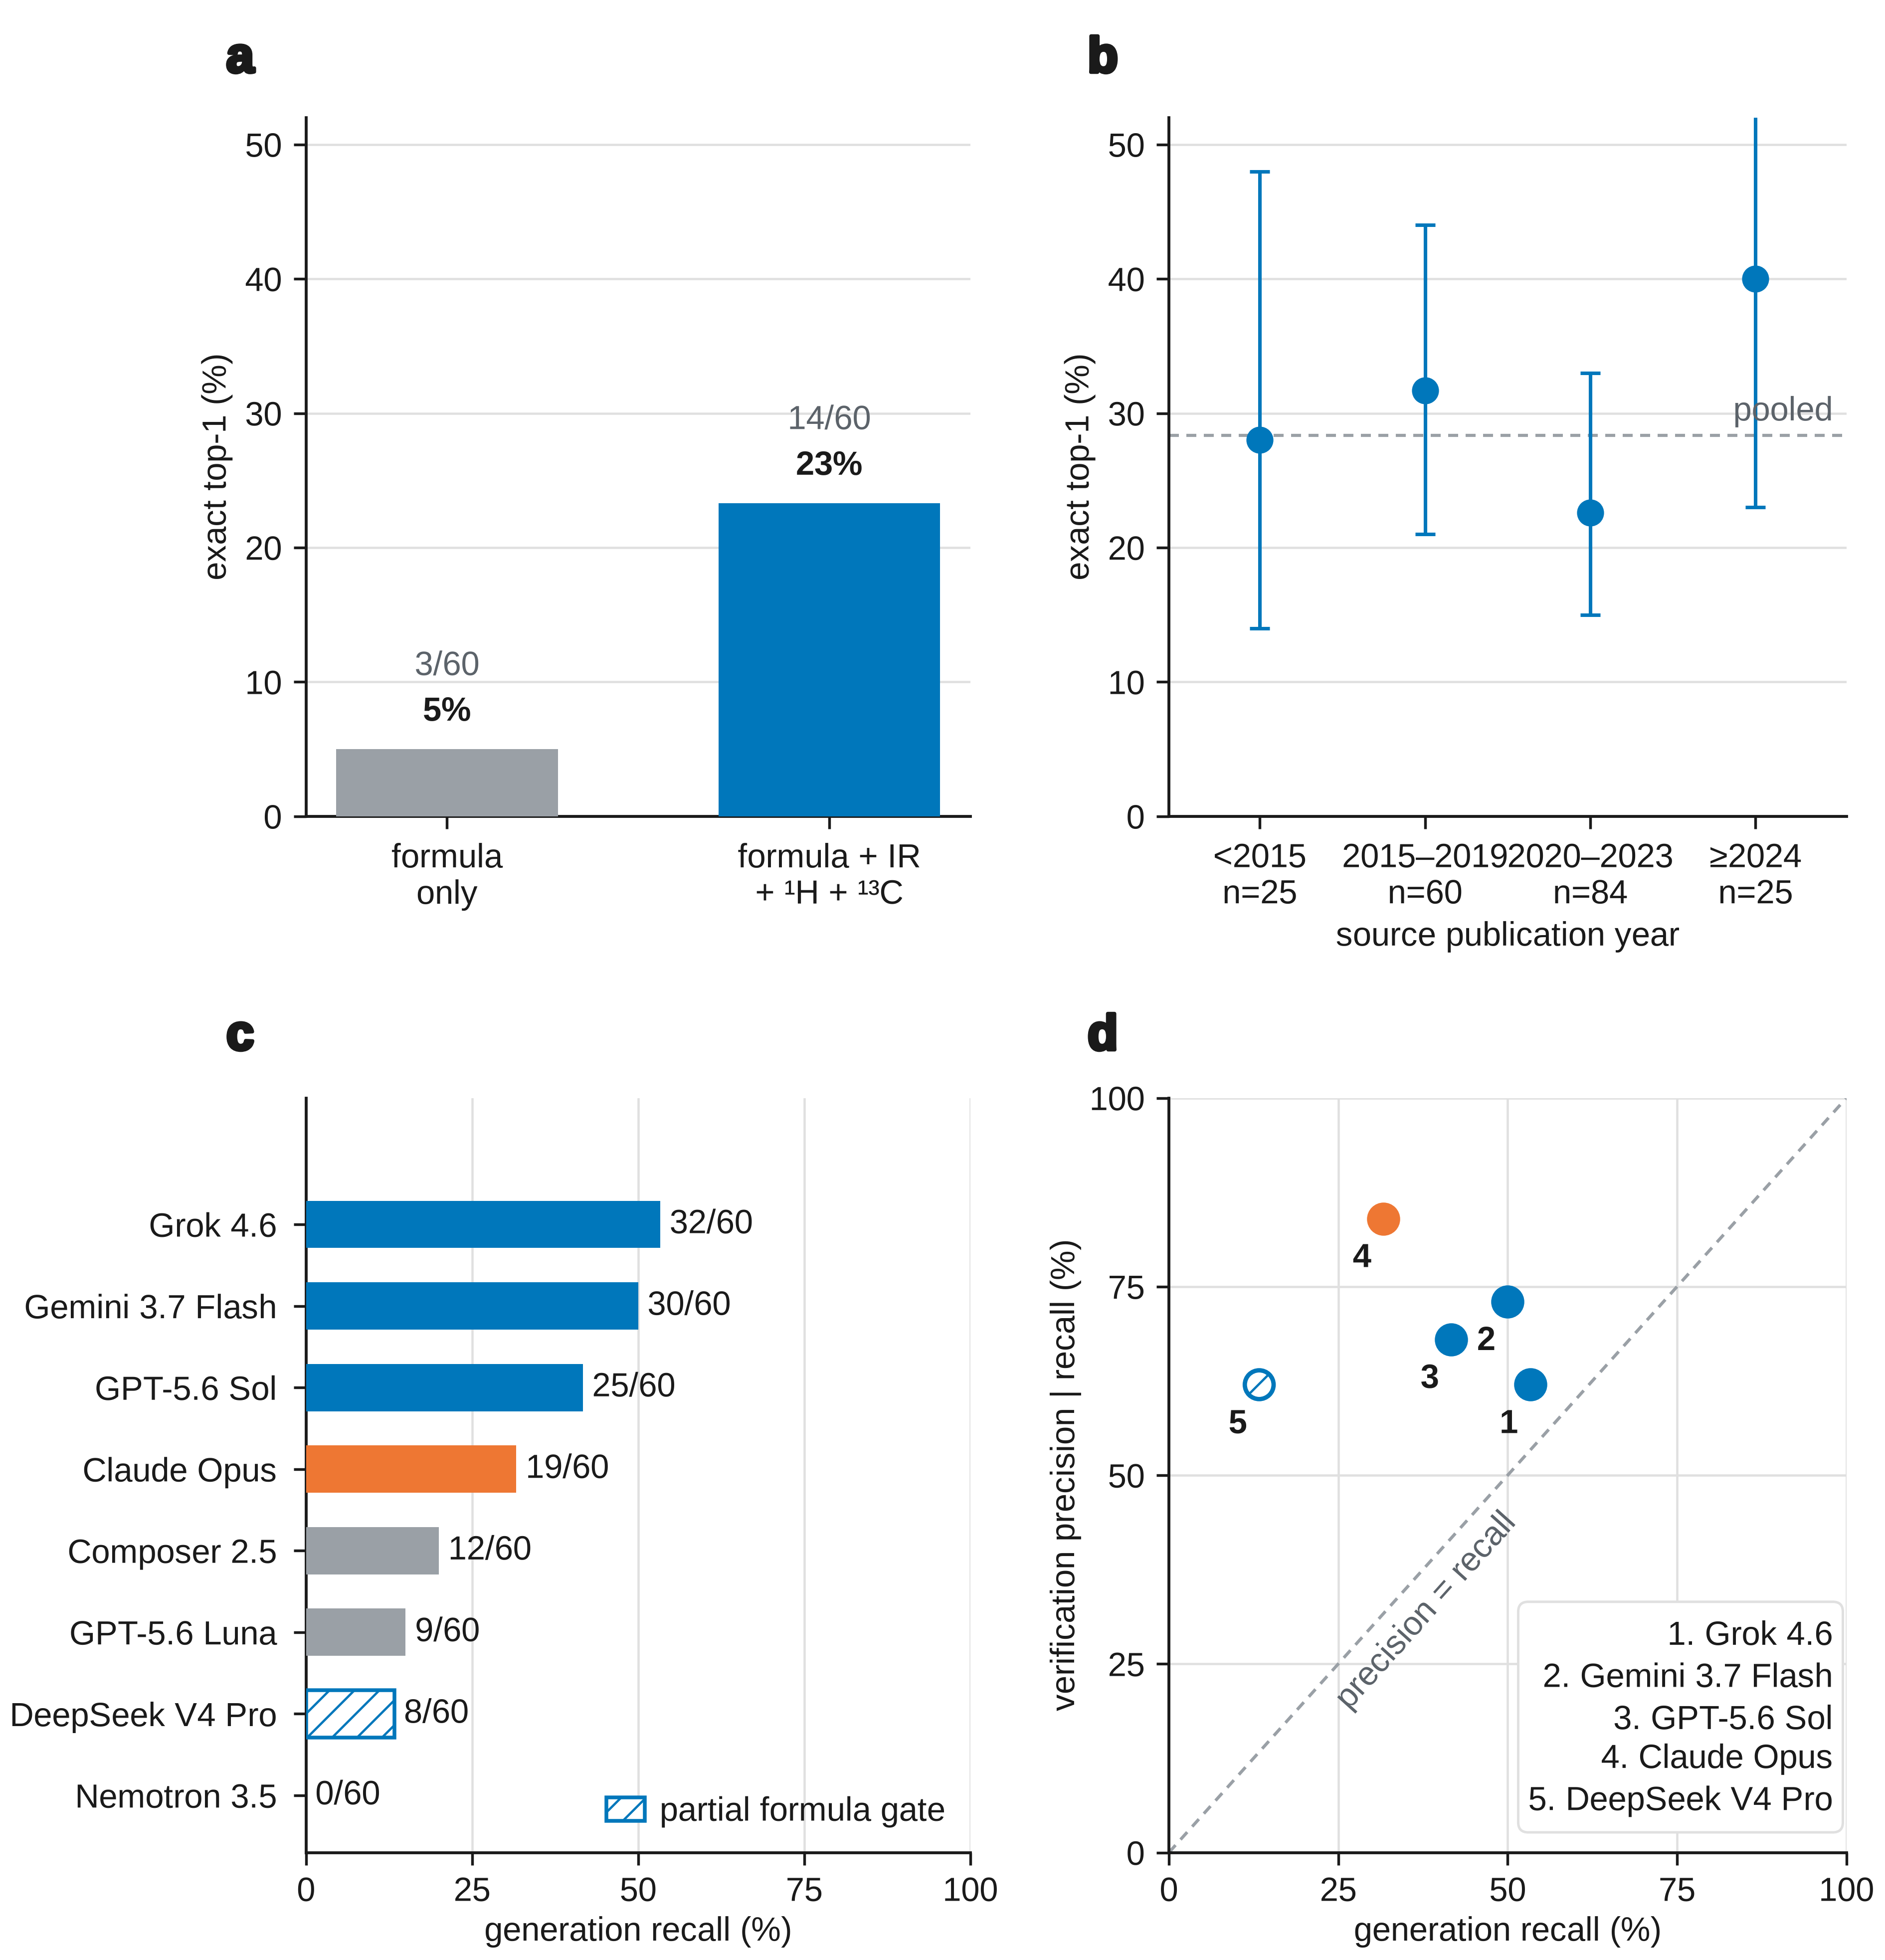
\includegraphics[width=\linewidth]{fig_robustness.png}
  \caption{Robustness of the recall-bound diagnosis: formula-only vs full modality; accuracy
  vs year; cross-vendor recall and precision.}
  \label{fig:fig-robustness}
\end{figure}

\subsection{Cross-vendor replication}
\label{sec:cross-vendor}

Grok 4.6, Gemini 3.7 Flash and GPT-5.6 Sol solved the same 60-compound arm under the
identical protocol.
\textbf{Verification precision exceeds generation recall in every arm}; bootstrapping
separates the paired gap for Claude (+52.5 points), GPT-5.6 Sol (+26.3) and Gemini (+23.3);
Grok's gap (+9.2) is directional.

\begin{table}[t]
\caption{Cross-vendor decomposition ($n{=}60$). Recall and precision have different
denominators --- the claim is the inequality, not a difference.}
\label{tab:cross-vendor}
\centering
\begin{tabular}{@{}lrrr@{}}
\toprule
model & generation recall & verification precision $|$ recall & multi-candidate only \\
\midrule
Claude Opus & 19/60 = 32\% & 16/19 = 84\% & 10/13 = 77\% \\
Grok 4.6 & 32/60 = 53\% & 20/32 = 62\% & 20/32 = 62\% \\
Gemini 3.7 Flash & 30/60 = 50\% & 22/30 = 73\% & 22/30 = 73\% \\
GPT-5.6 Sol & 25/60 = 42\% & 17/25 = 68\% & 16/24 = 67\% \\
\bottomrule
\end{tabular}
\end{table}

Candidate budgets differ (Claude mean 2.20 vs others 3.00), so recall rankings are
approximate.
A clean-clone control for Grok bounds key leakage (McNemar $p{=}0.39$).

\subsection{Forward-verification decomposition}
\label{sec:forward-verify}

\begin{figure}[t]
  \centering
  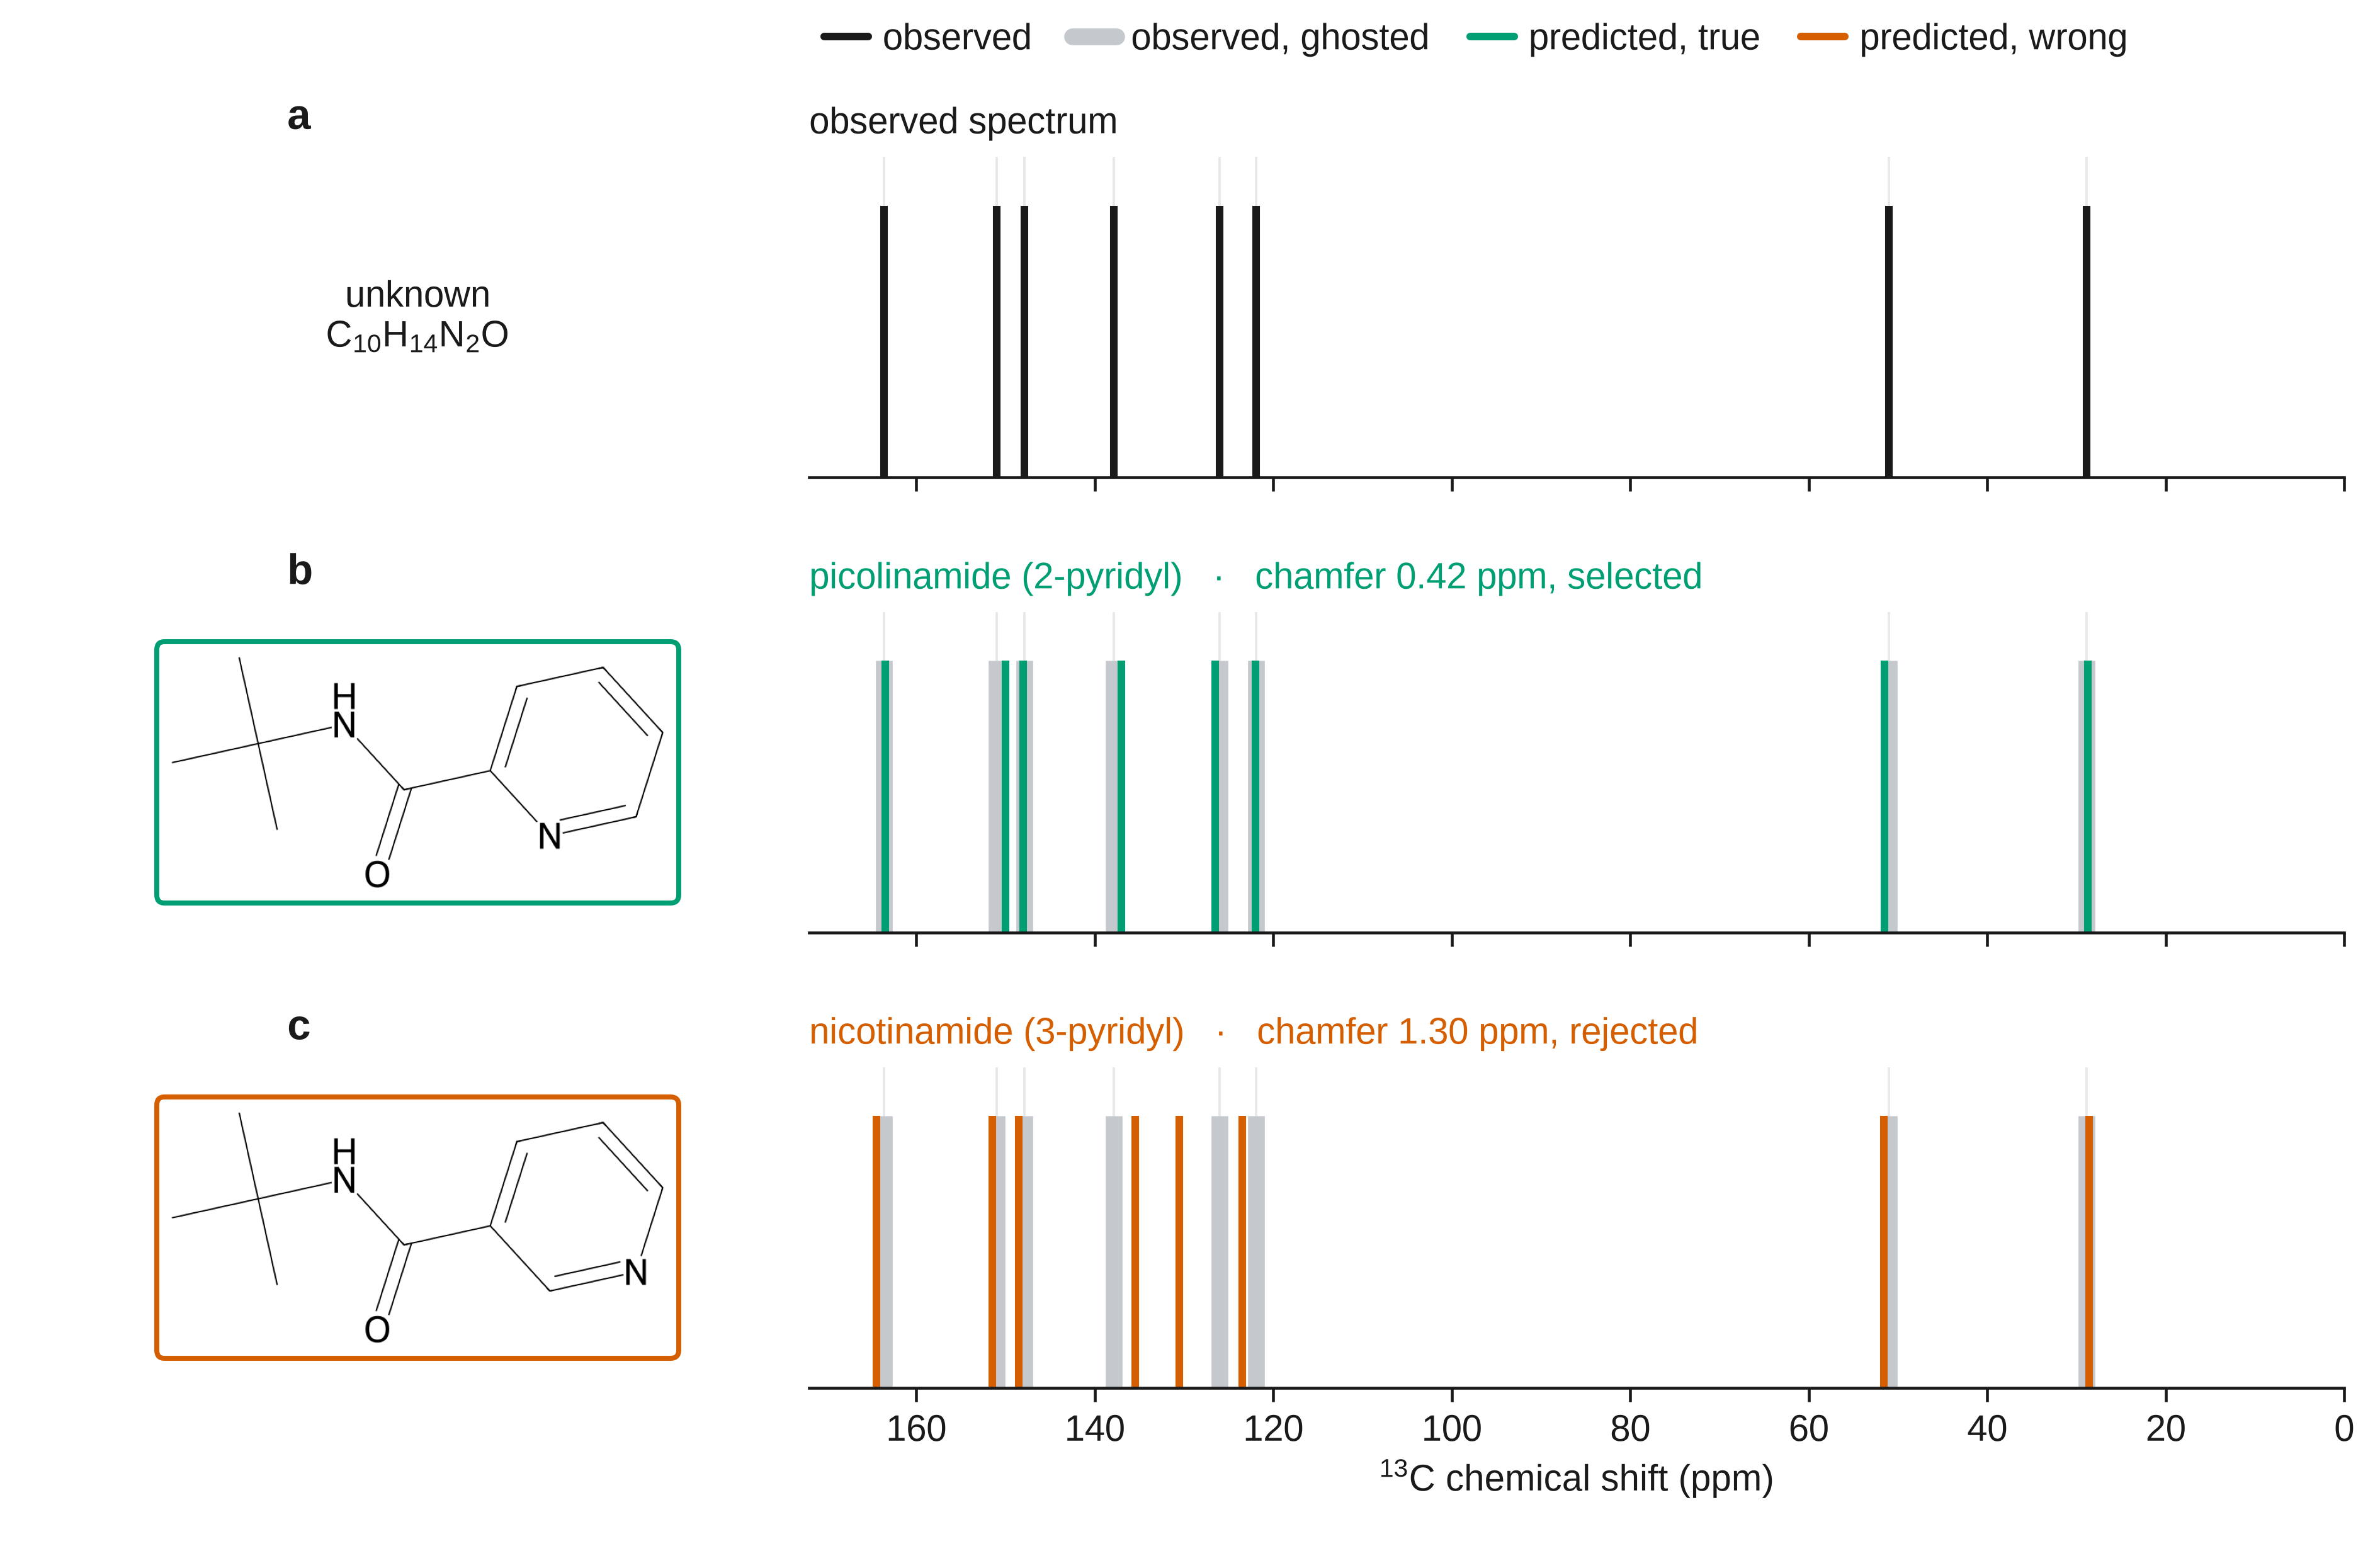
\includegraphics[width=0.92\linewidth]{fig_mechanism.png}
  \caption{Forward-verification on a regioisomer pair: inverse task is ambiguous;
  forward-predicted $^{13}$C separates isomers.}
  \label{fig:fig-mechanism}
\end{figure}

\begin{table}[t]
\caption{Forward-verification decomposition on the instrumented slice.
Expansion forward-verify has not been run; pooled $n{=}295$ numbers in
Table~\ref{tab:headline} are generation top-1 / recall only.}
\label{tab:fverify}
\centering
\begin{tabular}{@{}lrr@{}}
\toprule
 & 60-compound arm & locked slice ($n{=}194$) \\
\midrule
generation recall & 19/60 (32\%) & 65/194 (34\%) \\
top-1, solver self-ranking & 14/60 (23\%) & 55/194 (28\%) \\
top-1, forward-verified re-ranking & 16/60 (27\%) & 58/194 (30\%) \\
precision $|$ recall --- forward-verification & 16/19 (84\%) & 58/65 (\textbf{89\%}) \\
multi-candidate only --- forward-verification & 10/13 (77\%) & 30/37 (81\%) \\
\bottomrule
\end{tabular}
\end{table}

When the true structure is among the candidates, forward-verification selects it in 58/65
cases (89\%).
Where a choice existed ($n{=}37$), forward-verification is correct on 30/37 (81\%) against a
54.0\% derangement floor (+27.1 points).
The margin over self-ranking is \textbf{small and unresolved} (seven gained, four lost;
McNemar $p{=}0.55$) --- we do \textbf{not} claim an accuracy advance.
Precision is high while recall binds: no re-ranking repairs the 129/194 compounds on this
slice where the true structure was never proposed (Figure~\ref{fig:fig-wall}).

\paragraph{Generate-wide.}
Ten solver agents, up to six candidates each, pooled and re-ranked on the 60-compound arm:
recall 32\% $\to$ \textbf{42\%}, top-1 23\% $\to$ \textbf{30\%} (McNemar $p{=}0.34$);
verification precision falls 84\% $\to$ 72\%.
The training-free ceiling remains recall-limited.

\begin{figure}[t]
  \centering
  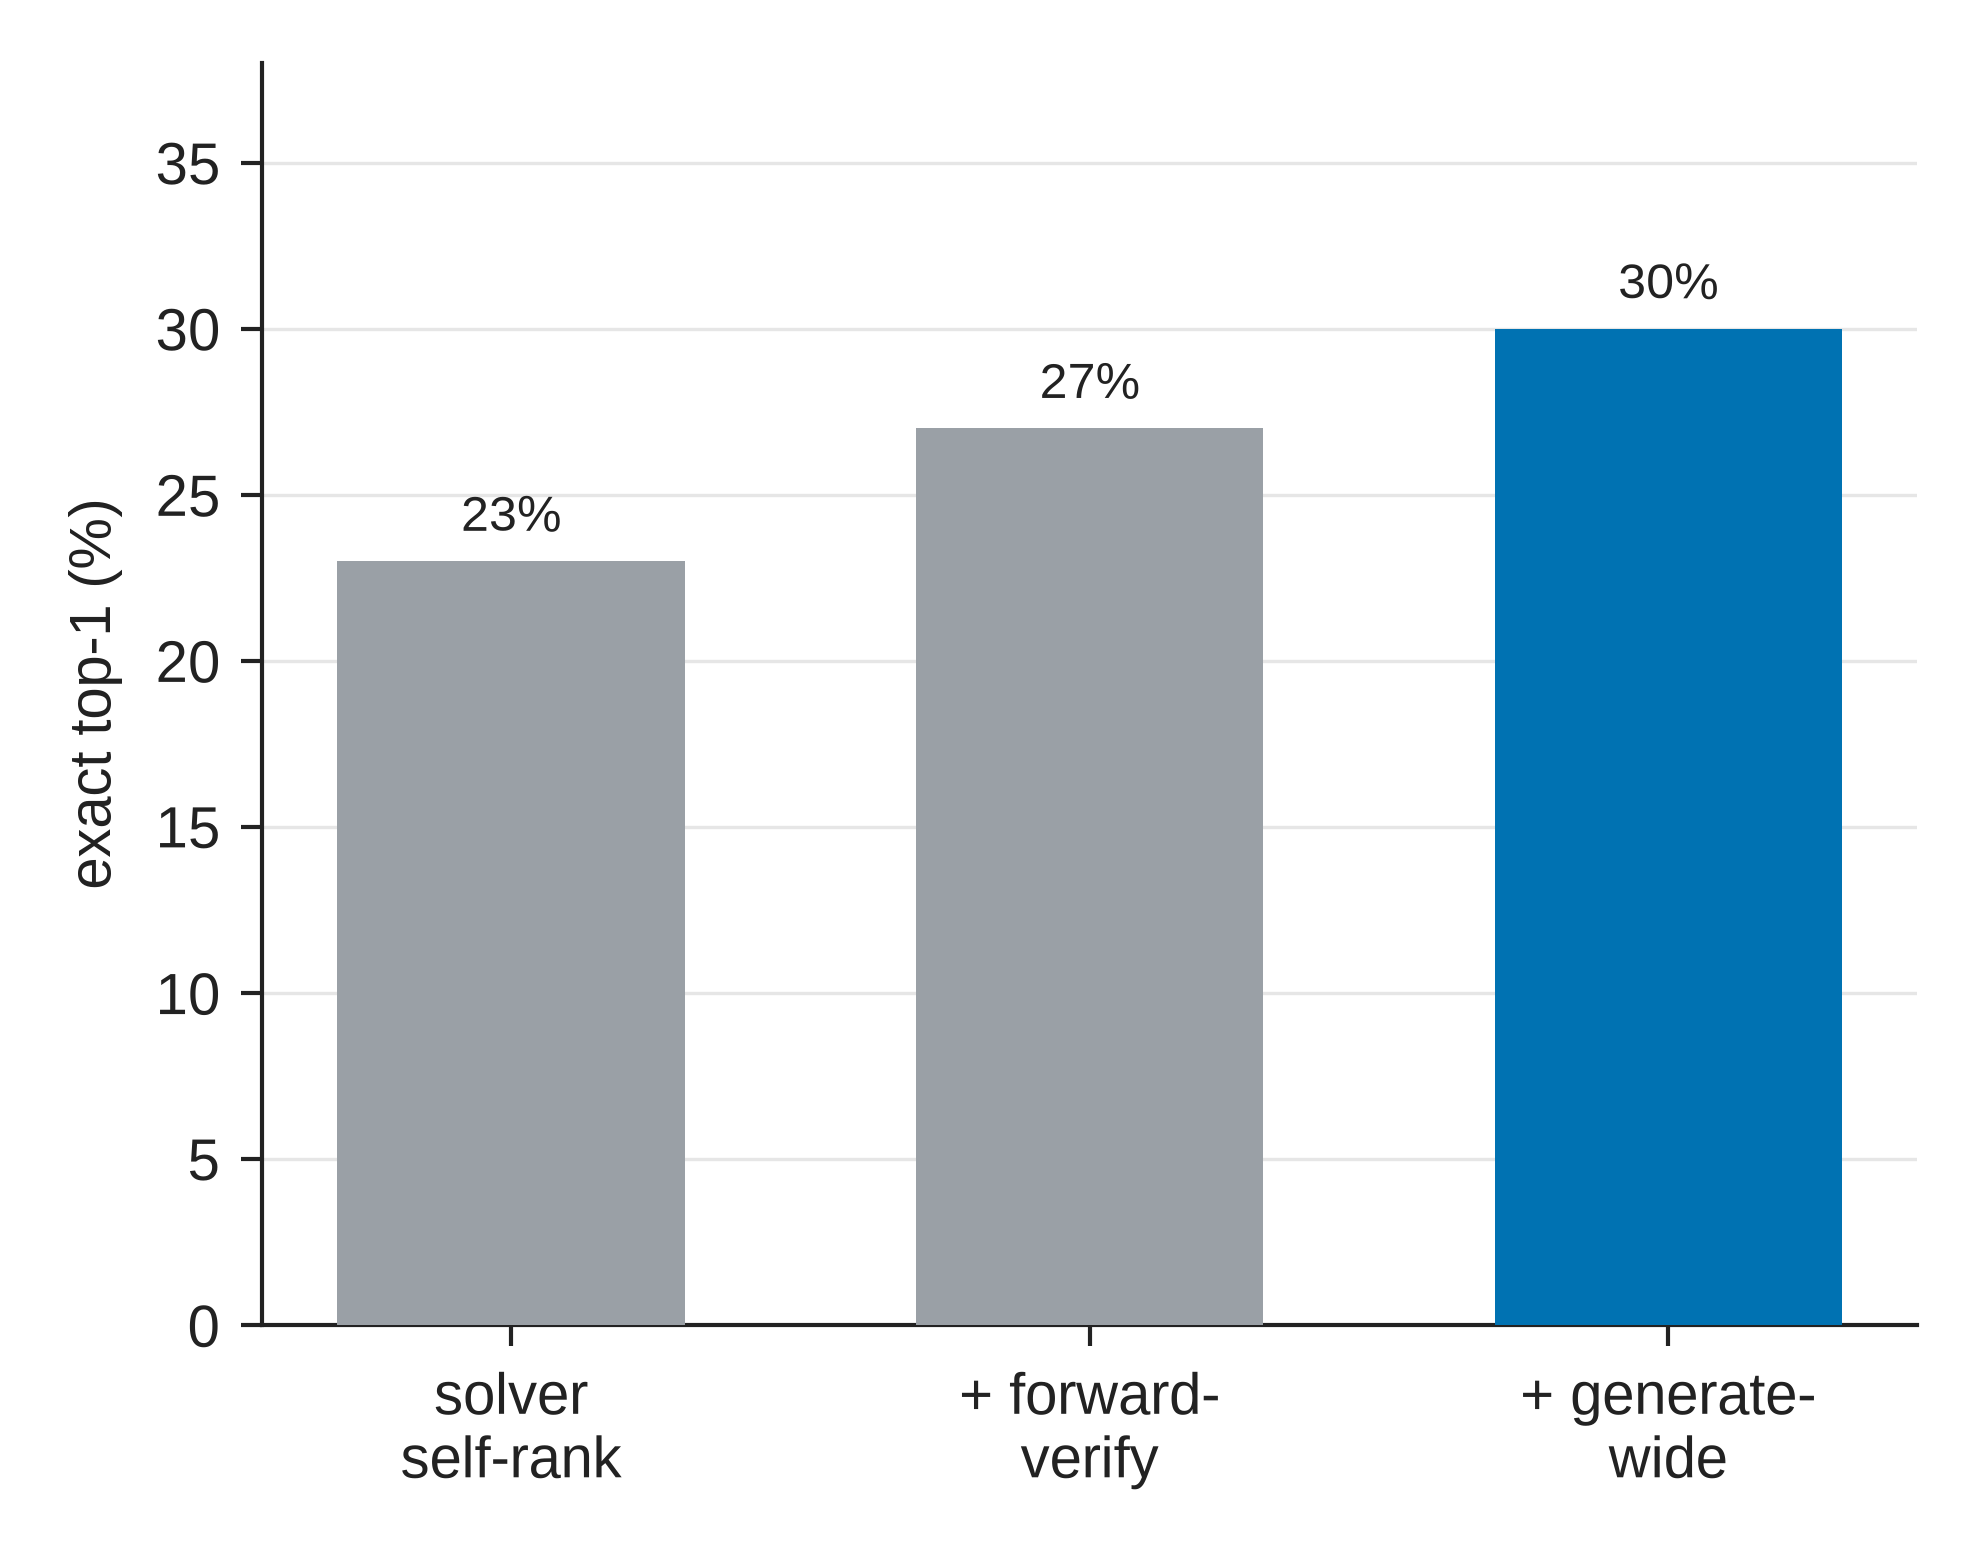
\includegraphics[width=\linewidth]{fig3_method.png}
  \caption{Forward-verification inference ladder on the 60-compound arm.}
  \label{fig:fig3-method}
\end{figure}

\paragraph{Non-LLM verifiers.}
On the same candidate sets, a HOSE-style lookup ties self-ranking; a modest GNN reaches
59/65 (91\%) vs the LLM verifier's 58/65 (89\%) --- directional.
Deranging observed $^{13}$C pairings collapses precision ($p{=}0.001$).
A small IRexp-fine-tuned generator pooled with Claude lifts locked-slice recall 33.5\% $\to$ 54.1\% and
top-1 28.4\% $\to$ 35.1\% (McNemar $p{=}0.015$), showing the wall is a property of
\textbf{training-free elicitation}, not of the task.

\subsection{Decomposition across published literature}
\label{sec:literature}

Any system reporting top-1 $= a$ and top-$k = b$ implies recall $\geq b$ and conditional
precision $\leq a/b$.
Applying this to published figures (\texttt{scripts/literature\_decomposition.py}):

\begin{table}[t]
\caption{Selected literature decomposition rows (connectivity-scored or as published).}
\label{tab:lit-decomp}
\centering
\scriptsize
\setlength{\tabcolsep}{3pt}
\begin{tabular}{@{}p{2.6cm}p{2.4cm}rrrr@{}}
\toprule
system & data ($n$) & top-1 & top-$k$ ($k$) & recall & prec. \\
\midrule
this work, solver alone & literature (295) & 39.3\% & 44.1\% (3) & 44.1\% & 89.2\% \\
this work + forward-verify & literature (194) & 29.9\% & 33.5\% (3) & 33.5\% & \textbf{89.2\%} \\
NMR-Solver~\citep{jin2025nmrsolver} & literature (450) & 52.9\% & 67.3\% (10) & $\geq$67.3\% & $\leq$78.6\% \\
NMRAgent~\citep{fang2026nmragent} & literature (450) & 61.6\% & 70.0\% (10) & $\geq$70.0\% & $\leq$88.0\% \\
Espejo Morales~\citep{espejo2026agentic} & education (236) & 80.9\% & 90.0\% (5) & $\geq$90.0\% & $\leq$89.9\% \\
Espejo Morales~\citep{espejo2026agentic} & industrial (34) & 20.6\% & 29.1\% (5) & $\geq$29.1\% & $\leq$70.9\% \\
Alberts, 6--13 atoms~\citep{alberts2025benchmarks} & NIST IR (3,455) & 63.8\% & 84.0\% (10) & 84.0\% & 75.9\% \\
SpecX, scaffold split~\citep{xiang2026specx} & simulated (99,439) & 29.7\% & 50.6\% (10) & 50.6\% & 58.7\% \\
\bottomrule
\end{tabular}
\end{table}

\textbf{Three groups changed only the data}, and recall carried \textbf{68\%} (NMR-Solver
simulated $\to$ real), \textbf{70\%} (SpecX random $\to$ scaffold) and \textbf{83\%}
(Espejo education $\to$ industrial) of each collapse.
Recall binds where spectra are real and heterogeneous; ranking dominates on simulated or
single-library data.
The solver-alone precision column on $n{=}295$ is self-ranking (116/130); the
forward-verify row is the instrumented $n{=}194$ slice (58/65). Those two 89.2\% figures
are not interchangeable: expansion forward-verify does not exist yet.

\subsection{Pre-registered expansion and the pooled headline}
\label{sec:expansion}

The $n{=}295$ headline is the pre-registered pool of the locked 194 and a 106-compound
expansion draw, after the same spectral-validation exclusion used on the main round
(Table~\ref{tab:slices}; Appendix Table~\ref{tab:expansion}).
Claude Opus recovers 63/106 (59.4\%) top-1 and 68/106 (64.2\%) generation recall on every
deposited expansion compound; 101/106 are spectrally clean (flags R12, R22, R25, R82, R91,
set before scoring), and the clean subset is 61/101 (60.4\%) / 65/101 (64.4\%).
Including the five flags (sensitivity $n{=}300$) is 118/300 (39.3\%) top-1 and 133/300 (44.3\%)
recall --- the one-decimal headline does not move; they are excluded because the stopping
rule says so.
The expansion slice is easier for this solver than the locked 194 (60.4\% vs 28.4\% top-1);
that gap is reported as found on a new draw, not hidden by pooling.
Forward-verification has \textbf{not} been run on the expansion, and a Fable cross-model arm
is incomplete (68/106 deposits, not scored, never pooled).
Figure~\ref{fig:fig-wall} and Table~\ref{tab:fverify} therefore remain the $n{=}194$
forward-verified diagnosis.

\section{Discussion}
\label{sec:discussion}

Frontier LLMs are \textbf{good verifiers} ($\approx$89\% conditional precision on the
$n{=}194$ forward-verified slice) and \textbf{weak proposers} (44\% generation recall on
$n{=}295$; 34\% on the instrumented 194) on real literature peak lists.
The primary research contribution of this paper is the \textbf{benchmark + stage
decomposition + contamination/cross-vendor diagnosis}, not a solved elucidator and not a
Data Descriptor for IRexp.
The expansion slice scored higher than the locked 194 (Section~\ref{sec:expansion}); pooling
does not erase that gap, and expansion forward-verify is still pending.

\paragraph{Reporting contract.}
External work on IRSpectra-Bench should deposit ranked SMILES under the released protocol and
report, at minimum: (i) top-1 constitution, (ii) generation recall, (iii) verification
precision $|$ recall, with bootstrap CIs and candidate budget.
Top-1 alone conflates the two stages.
Nonsignificant ladder gains (forward-verification vs self-ranking, $p{=}0.55$; generate-wide
top-1, $p{=}0.34$) should be cited as \textbf{diagnostic}, not as accuracy advances.
Corpus-reweighted top-1 (\textbf{26.5\%}) is the better estimate for an arbitrary literature
draw.

Training is not foreclosed: IRexp fine-tuning lifts recall to 54\%.
Those gains compound with open experimental data, honest benchmarks, and inference scaffolding that
transfers to each new model.

\section{Limitations}
\label{sec:limitations}

Scoring is mechanical; solver runs were transcript-audited for zero ground-truth access.
\textbf{(i) Consumer harness.} No model snapshot, temperature, seed or thinking tier; exact
inference is not reproducible. Scoring is. Instruction text wrapping Claude batches was not
captured --- only per-compound payloads are released.
\textbf{(ii) Pretraining contamination} is bounded by formula-only (23\% $\to$ 5\%) and flat
recency but \textbf{not excluded}; verbatim spectral strings from PMC in the prompt remain a
retrieval confound.
\textbf{(iii) Object type, formula and scoring.} Band/shift lists, not raw traces; formula
supplied (as from HRMS) --- absolute accuracies are not interchangeable with no-formula
systems. Headline metrics score constitution; with stereochemistry, top-1 is 93/295 (31.5\%).
\textbf{(iv) Statistical honesty.} Forward-verification vs self-ranking unresolved ($p{=}0.55$);
generate-wide top-1 likewise ($p{=}0.34$). Four-model comparison at $n{=}24$ underpowered for
adjacent ranks with disclosed protocol asymmetry. The inference ladder \textbf{diagnoses a
bottleneck}; it is not a demonstrated accuracy advance.
\textbf{(v) Missing on-bench cheminformatics baselines.} Spectro, NMIRacle, Alberts IR
transformers and CASE were \textbf{not scored} on IRSpectra-Bench --- the LLM recall wall is
not cleanly separated from harness or modality choice.
\textbf{(vi) Cross-vendor scope.} Headline $n{=}295$ is Claude Opus generation; four-vendor replication is
on 60 compounds; candidate budgets differ.
Forward-verification, Figure~\ref{fig:fig-wall}, and verification precision $|$ recall (58/65)
are the locked $n{=}194$ slice --- expansion forward-verify is pending.
A Fable cross-model arm on the expansion draw is incomplete (68/106) and is not pooled.
\textbf{(vii) Deferred arms.} Expert-chemist audit of elucidation outputs formally deferred
(not run). Leave-one-modality-out ablation abandoned for this manuscript. Extraction-recall
human audit of the mining parser is deferred to the \textit{Scientific Data} companion.
\textbf{(viii) Scope.} Battery subset uses literature electrolyte chemistry, not operando
spectra; single-sample scoring per compound; organic literature bias of PMC-OA sources.

\section{Conclusion}
\label{sec:conclusion}

IRSpectra-Bench makes LLM structure elucidation from literature peak lists \textbf{measurable
and decomposable}.
On that protocol, generation recall --- not verification --- binds end-to-end accuracy; the
diagnosis replicates across vendors and is recovered from published top-$k$ figures.
We release frozen predictions and a mechanical scorer so others can report the same three
numbers.
The redistributable experimental band-list corpus behind the bench is documented separately
as a \textit{Scientific Data} Data Descriptor (in preparation)~\citep{yabbarov2026irexp}, with an
anonymised review copy linked in Appendix~\ref{app:dataset}.

\section*{Reproducibility statement}
Every training-free number regenerates from released questions, answers, frozen predictions
and scripts in the code release.
The sampler, InChIKey scorer and forward-verification harness are scripted end-to-end.
Consumer-harness inference cannot be bit-exact replayed (Section~\ref{sec:limitations});
distributional agreement is the intended claim.
Fine-tuning against the bench should use \texttt{data/train\_no\_bench.jsonl.gz} so benchmark
InChIKeys are withheld.

\section*{Ethics statement}
This work evaluates publicly available open-access literature peak lists and commercial LLM
APIs under consumer terms.
No human-subject data.
We do not claim clinical or regulatory readiness for automated elucidation.
Licensing of redistributed numeric extractions is documented in the companion Data Descriptor
and dataset notices (PMC-OA terms are mixed --- not uniformly CC-BY; Chemotion is CC-BY-SA).

\section*{Acknowledgements}
We acknowledge support from the Natural Sciences and Engineering Research Council of Canada (NSERC) through a CREATE training program. Institutional details and named funding references are omitted for double-blind review and will be restored in the camera-ready version.
\bibliography{references}
\bibliographystyle{iclr2026_conference}

\appendix

\section{Dataset pointer (IRexp)}
\label{app:dataset}

IRexp is \textbf{not} re-described here as a Data Descriptor.
During double-blind review, the commercial redistributable pool is available from an anonymised review copy (no author-identifying host):
\begin{itemize}
  \item Anonymised dataset copy: \url{https://anonymous.4open.science/r/peaklist-corpus-review-10C4/}
  \item Companion manuscript: anonymised \textit{Scientific Data} Data Descriptor (in preparation)~\citep{yabbarov2026irexp}
\end{itemize}
Named archival hosting will replace the review copy in the camera-ready version.
File schema and aggregate counts ship with that copy (\texttt{SCHEMA.md}, \texttt{data/}).

Benchmark construction details beyond Section~\ref{sec:benchmark} (spectral validation
filters, prompt-leakage audit, electrolyte SMARTS) ship with the code release and the
companion Data Descriptor~\citep{yabbarov2026irexp}; they are not re-presented here.

\section{Extended tables and figures}

This conference version keeps four main-text figures: the diagnosis wall
(Figure~\ref{fig:fig-wall}), robustness (Figure~\ref{fig:fig-robustness}), the
forward-verification mechanism (Figure~\ref{fig:fig-mechanism}), and the inference
ladder (Figure~\ref{fig:fig3-method}).
Additional archive plates are omitted here; they do not change the pooled $n{=}295$
generation headline or the $n{=}194$ forward-verified wall.

\begin{table}[h]
\caption{Expansion round (Claude Opus, InChIKey-14). Headline $n{=}295$ excludes the five
$^{13}$C-overread flags. Forward-verification has not been run; a Fable arm is incomplete
(68/106) and is never pooled. Sensitivity $n{=}300$ (including flags) is 118/300 (39.3\%)
top-1 and 133/300 (44.3\%) recall.}
\label{tab:expansion}
\centering
\begin{tabular}{@{}lrr@{}}
\toprule
 & all ($n{=}106$) & clean ($n{=}101$) \\
\midrule
top-1 & 63/106 (59.4\%) & 61/101 (60.4\%) \\
generation recall & 68/106 (64.2\%) & 65/101 (64.4\%) \\
\bottomrule
\end{tabular}
\end{table}

\end{document}
